%  !TeX  root  =  user_guide.tex

\section{Модуль GPS}\label{label_plugingps}

% when the revision of a section has been finalized,
% comment out the following line:
% \updatedisclaimer

\subsection{Что такое GPS?}\label{whatsgps}

GPS, система глобального позиционирования, "--- это спутниковая система,
которая позволяет любому имеющему GPS приёмник найти свое точное
местоположение где бы то ни было на планете. Используется в качестве
вспомогательного устройства в навигации, к примеру, в самолетах, на
кораблях и просто путешественниками. GPS приемник использует сигналы со
спутников для просчёта широты, долготы и (иногда) высоты. Большинство
приёмников также могут хранить точки (также известные, как
\emph{маршрутные точки}), последовательности точек, составляющих
запланированный \emph{маршрут} и лог трека или просто \emph{трек}
движения приемника на протяжении времени. Маршрутные точки, маршруты и
треки являются тремя базовыми типами GPS данных. QGIS отображает
маршрутные точки на точечных слоях, тогда как маршруты и треки
показываются на линейных слоях.

\subsection{Загрузка GPS данных из файла}\label{label_loadgps}

Существуют десятки различных форматов файлов для хранения GPS данных.
Формат, используемый в QGIS, называется GPX (формат обмена данными GPS),
являющийся стандартным обменным форматом, который может содержать любое
количество маршрутных точек, маршрутов и треков в одном файле.

Для того, чтобы загрузить GPX файл, сначала нужно загрузить модуль.
\mainmenuopt{Модули} \arrow
\dropmenuopttwo{mActionShowPluginManager}{Управление модулями} \arrow
\checkbox{Инструменты GPS}.
Когда модуль загружен, на панели инструментов появится иконка с
небольшим ручным GPS устройством. В наборе сэмплов QGIS присутствует
пример GPX файла: \\
\filename{/qgis\_sample\_data/gps/national\_monuments.gpx}.
Смотрите Раздел~\ref{label_sampledata} для более детальной информации
о сэмплах.

\begin{enumerate}
\item Нажмите кнопку \toolbtntwo{gps_importer}{Инструменты GPS} и
откройте закладку \tab{GPX-файлы} (см. Рисунок~\ref{fig:gpxloader}).
\item Используйте кнопку \button{Обзор} для перехода в каталог
\filename{qgis\_sample\_data/gps/}, выберите файл GPX
\filename{national\_monuments.gpx} и нажмите кнопку \button{Открыть}.
\end{enumerate}

\begin{figure}[ht]
   \centering
   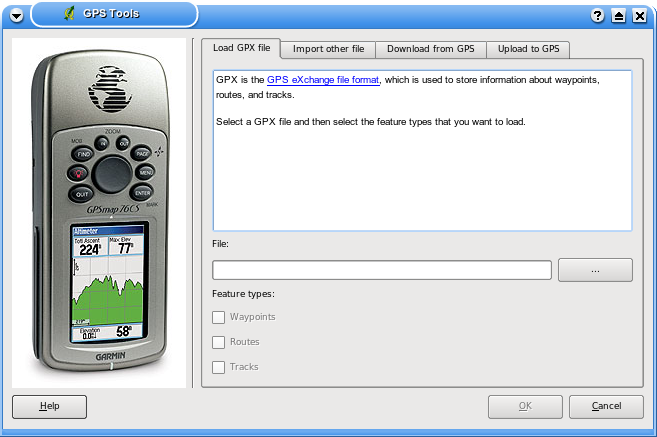
\includegraphics[clip=true, width=12cm]{loadgpx}
   \caption{Диалоговое окно \emph{Инструменты GPS} \nixcaption}\label{gpxloader}
\end{figure}

Следует использовать кнопку \browsebutton для того, чтобы выбрать файл
GPX, затем установить флаги для выбора типов объектов, которые нужно
загрузить из этого файла GPX. Каждый тип объектов будет загружен в
отдельный слой, как только вы нажмете кнопку \button{OK}. Файл
\filename{national\_monuments.gpx} включает лишь маршрутные точки.

\subsection{Программа GPSBabel}

Так как QGIS работает с файлами GPX, нужен способ конвертирования других
форматов GPS файлов в GPX. Это возможно благодаря свободно
распространяемой программе GPSBabel, которая доступна на сайте
\url{http://www.gpsbabel.org}. Эта программа может также передавать
данные GPS между компьютером и устройством GPS. QGIS использует GPSBabel
для подобного рода операций, поэтому рекомендуется установить последнюю
версию этой программы на ваш компьютер. Тем не менее, если нужно только
загрузить данные GPS из файлов GPX, эта программа не понадобится.
GPSBabel версии 1.2.3 совместима с QGIS, но использование более поздних
версий не должно вызвать каких-либо сложностей.

\subsection{Импортирование данных GPS}

Для того, чтобы импортировать данные GPS из файла, не являющегося файлом
GPX, нужно перейти на вкладку \tab{Прочие файлы} в диалоговом окне
\dialog{Инструменты GPS}. Здесь можно выбрать файл для импортирования
(а также тип файла), какой тип объектов нужно импортировать, куда нужно
сохранить cконвертированный файл GPX и какое имя надо присвоить новому
слою. Заметьте, что не все форматы данных GPS будут поддерживать все
три типа объектов, поэтому для многих форматов можно выбрать только один
или два типа.

\subsection{Загрузка данных GPS из устройства}

QGIS может использовать GPSBabel для непосредственной загрузки данных из
устройства GPS в качестве новых векторных слоев. Для этого предназначена
закладка \tab{Загрузка с GPS} в диалоговом окне \dialog{Инструменты GPS}
(см. Рисунок~\ref{figure_download}). Здесь выбирается тип устройства,
порт, к которому оно подключено, тип объектов для загрузки, файл GPX, в
который данные должны быть сохранены, а также название нового слоя.

\begin{figure}[ht]
   \centering
   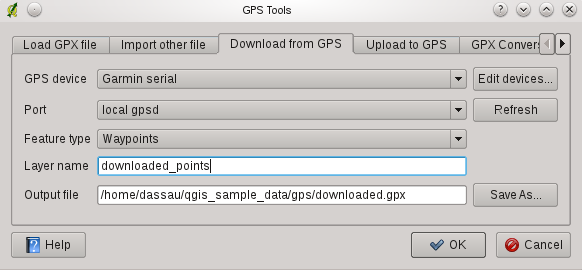
\includegraphics[clip=true, width=12cm]{download}
   \caption{Инструмент загрузки \nixcaption}\label{figure_download}
\end{figure}

Тип устройства, выбираемый в меню устройства GPS, определяет, как
GPSBabel попытается соединиться с устройтвом. Если ни один тип из
имеющихся не подходит вашему устройству, можно создать новый тип
(см. Раздел~\ref{sec:Defining-new-device}).

Порт может быть названием файла или каким-то другим названием, которое
операционная система использует в качестве ссылки на физический порт в
компьютере, к которому подключено устройство GPS. Это может быть
обычный USB, для устройств, его поддерживающих.
\nix В Линуксе таким может быть /dev/ttyS0 или /dev/ttyS1, а в
\win Windows "--- это COM1 или COM2.

После нажатия кнопки \button{OK}, данные загрузятся с устройства и
появятся в QGIS в качестве слоя.

\subsection{Загрузка данных GPS в устройство}

Кроме того, можно загрузить данные из векторного слоя в QGIS
непосредственно в устройство GPS, используя закладку \tab{Выгрузка в GPS}
диалогового окна \dialog{Инструменты GPS}. Чтобы сделать это, нужно просто
выбрать слой для выгрузки (являющийся слоем GPX), тип устройства GPS и
порт, к которому оно подключено. Так же, как и в инструменте загрузки
из GPS, можно выбрать новые типы устройств, если ваше устройство
отсутствует в списке.

Этот инструмент очень полезен при совместном использовании с
инструментами редактирования векторных данных QGIS. Это дает возможность
загрузить карту, создать маршрутные точки и маршруты, а затем выгрузить
их в GPS навигатор.

\subsection{Определение новых типов устройств}\label{sec:Defining-new-device}

Существует множество различных типов устройств GPS. Разработчики QGIS не
могут протестировать их все, поэтому, если у вас одно из тех, что не
работают ни с одним из типов устройств в списке в закладках
\tab{Загрузка с GPS} и \tab{Выгрузка в GPS}, можно определить ваш
собственный тип устройства. Сделать это можно, обратившись в редактору
устройств GPS, который вызывается по нажатию кнопки \\
\button{Редактировать устройства} в обеих закладках.

Для того, чтобы определить устройства, нужно просто нажать кнопку
\button{Создать}, ввести название, команду загрузки и выгрузки для
вашего устройства, а также нажать кнопку \button{Обновить}. Название
появится в меню обеих закладок и может быть любой последовательностью
символов. Командой загрузки является команда, используемая для загрузки
данных из устройства в файл GPX. Скорее всего, это будет команда
GPSBabel, но существует возможность использовать любую другую программу
командной строки, которая может создавать файл GPX. QGIS заменит
ключевые слова \usertext{\%type}, \usertext{\%in} и
\usertext{\%out}, когда команда будет запущена на выполнение.

\usertext{\%type} будет заменено на {}``\usertext{-w}'' в случае,
если загружаются маршрутные точки, {}``\usertext{-r}'', если
загружаются маршруты и {}``\usertext{-t}'', если загружаются треки.
Эти параметры говорят GPSBabel, какой тип объектов загружать.

\usertext{\%in} будет заменено на название порта, выбранного в окне
<<Загрузка с GPS>> и \usertext{\%out} заменится на название, выбранное
для файла GPX, в котором будут сохраняться загруженные данные. Таким
образом, если создается тип устройства с командой загрузки
{}``\usertext{gpsbabel \%type -i garmin -o gpx \%in \%out}'' (это
фактически команда загрузки для предопределённого типа устройств
\selectstring{GPS-устройство:}{Garmin serial}), а затем используется
для загрузки маршрутных точек через порт {}``\usertext{/dev/ttyS0}'' с
сохранением в файл {}``\usertext{output.gpx}'', QGIS заменит ключевые
слова и запустит команду \\
{}``\usertext{gpsbabel -w -i garmin -o gpx /dev/ttyS0 output.gpx}''.

Команда выгрузки "--- это команда, применяемая для выгрузки данных в
устройство. В ней применяются те же ключевые слова, однако
\usertext{\%in} уже заменяется на название файла GPX для выгруженного
слоя, а \usertext{\%out} заменяется на название порта.

Более подробную информацию о программе GPSBabel и другие ее параметры
запуска можно найти на сайте \url{http://www.gpsbabel.org}.

Как только новый тип устройства будет создан, он появится в списках
устройств в обеих закладках окна \dialog{Инструменты GPS} "-- \tab{Загрузка с GPS}
и \tab{Выгрузка в GPS}.

\FloatBarrier
